本节,我们证明两个十分重要的定理. 它们分别刻画了紧空间上的连续函数空间的紧子集与稠密子集.

\mysubsection{Arzelà-Ascoli 定理}

\begin{definition}
    设 $X$ 为集合,$(Y,\rho)$ 为度量空间. 设 $\mathscr{F}=\set{f:X\to Y}$ 为一族函数.

    称 $\mathscr{F}$ 一致有界,若所有 $f\in\mathscr{F}$ 的值域之并在 $Y$ 中有界. 即
$$
V\triangleq\set{f(x)|x\in X,f\in\mathscr{F}}
$$

    在 $Y$ 中有界.

    称 $\mathscr{F}$ 完全有界,若 $V$ 是 $Y$ 中的完全有界集.
\end{definition}

\begin{hint}
    若 $Y=\RR^n$ 或 $\mathbb{C}^n$,则 $A\subset Y$ 有界 $\iff A$ 完全有界.

    从而在此时函数族 $\mathscr{F}$ 一致有界与完全有界等价.

    但若 $Y$ 为无穷维赋范线性空间,则完全有界的概念严格强于有界. 例如 $Y=C[a,b]$.
\end{hint}

\begin{definition}
    设 $(X,d),(Y,\rho)$ 均为度量空间,$\mathscr{F}=\set{f:X\to Y}$ 为一族函数.

    称 $\mathscr{F}$ 等度连续,若
$$
\forall\eps>0,\exists\delta>0,\forall x_1,x_2\in X,d(x_1,x_2)<\delta\implies\forall f\in\mathscr{F},\rho(f(x_1),f(x_2))<\eps
$$
\end{definition}

\begin{example}
    $\mathscr{F}=\set{x^n|n\ge 1},X=[0,1]$.

    则 $\mathscr{F}$ 一致有界,但不等度连续.
\end{example}

\begin{example}
    $\mathscr{F}=\set{\sin nx|n\in\mathbb{N}}$ 在任何区间 $[a,b]$ 上均不等度连续.
\end{example}

\begin{example}
    若 $\mathscr{F}$ 是一族从 $\RR$ 到 $\RR$ 的映射,且
$$
\exists L>0,\forall f\in\mathscr{F},\forall x,y\in\RR,\abs{f(x)-f(y)}\le L\abs{x-y}
$$

    则 $\mathscr{F}$ 等度连续.
\end{example}

如上的概念与一致收敛性有密切的连续:

\begin{lemma}
    设 $K$ 为紧度量空间,$Y$ 为完备度量空间.

    设 $f_n\in C(K;Y)$. 若 $\set{f_n}$ 在 $K$ 上一致收敛,则 $\set{f_n}$ 在 $K$ 上完全有界且等度连续.
\end{lemma}
\begin{proof}
    设 $f_n\rightrightarrows f:K\to Y$. 则 $f$ 也连续.

    \begin{itemize}
        \item 完全有界:
        
        由 $f_n,f$ 连续且 $K$ 紧知 $f_n(K),f(K)$ 均为 $Y$ 中的紧集. 从而完全有界. 由 $f(K)$ 完全有界知
$$
\forall\eps>0,\exists x_1,\cdots,x_k\in K,f(K)\subset\bigcup_{j=1}^kB\left(f(x_j),\frac{\eps}{2}\right)
$$

        由 $f_n\rightrightarrows f$ 知
$$
\begin{aligned}
    \exists N\in\mathbb{N},\forall n\ge N,&\forall x\in K,\abs{f_n(x)-f(x)}<\frac{\eps}{2}\\
    \implies&f_n(K)\subset\bigcup_{j=1}^kB(f(x_j),\eps)
\end{aligned}
$$

        故 $\bigcup\limits_{n\ge N}f_n(K)$ 完全有界.

        由 $f_1(K)\cup\cdots\cup f_N(K)$ 是有限个完全有界集之并,知其完全有界. 故
$$
V\triangleq\bigcup_{n=1}^\infty f_n(K)=\bigcup_{n=1}^Nf_n(K)\cup\bigcup_{n\ge N}f_n(K)
$$

        完全有界. 即 $\set{f_n}$ 完全有界.
        
        \item 等度连续:
        
        任取 $\eps>0$. 由 $f_n\rightrightarrows f$ 知
$$
\exists N\in\mathbb{N},\forall n\ge N,\forall x\in K,\abs{f_n(x)-f(x)}<\frac{\eps}{3}
$$

        由 $f_1,\cdots,f_N,f$ 在紧集 $K$ 上连续知它们一致连续. 从而
$$
\begin{aligned}
    \exists\delta>0,\forall x,x'\in K,d(x,x')<\delta\implies&\rho(f_j(x),f_j(x'))<\frac{\eps}{3},1\le j\le N\\
    &\rho(f(x),f(x'))<\frac{\eps}{3}
\end{aligned}
$$

        则对 $n\ge N$ 有
$$
\begin{aligned}
    \forall x,x'\in K,d(x,x')<\delta\implies&\rho(f_n(x),f_n(x'))\\
    \le&\rho(f_n(x),f(x))+\rho(f(x),f(x'))+\rho(f(x'),f_n(x'))\\
    <&\frac{\eps}{3}+\frac{\eps}{3}+\frac{\eps}{3}=\eps
\end{aligned}
$$

        即 $\set{f_n}$ 等度连续.
    \end{itemize}
\end{proof}

现在我们可以陈述 Arzelà-Ascoli 定理.

\begin{theorem}[Arzelà-Ascoli]
    设 $\mathscr{F}$ 是一族从紧度量空间 $K$ 到完备度量空间 $Y$ 的函数. 则

    $\forall\set{f_n}\subset\mathscr{F}$,存在子列 $n_k$ 使得 $\set{f_{n_k}}$ 一致收敛 $\iff\mathscr{F}$ 完全有界且等度连续.
\end{theorem}
\begin{proof}
    $\implies$:反证,设 $\mathscr{F}$ 不完全有界,即 $V=\set{f(x)|x\in K,f\in\mathscr{F}}$ 不完全有界.
    
    即存在 $\eps_0>0$ 使得 $V$ 不存在有限 $\eps_0$-网.

    则可以构造 $f_n\in\mathscr{F},x_n\in K$ 满足
$$
\rho(f_n(x_n),f_m(x_m))\ge\eps_0,\forall n\ne m
$$

    这说明 $\set{f_n}\subset\mathscr{F}$ 不完全有界,且 $\set{f_n}$ 的任何子列也不完全有界. 从而由引理知其不可能一致收敛.

    反证,设 $\mathscr{F}$ 不等度连续.

    则存在 $\eps_0>0$ 以及 $f_n\in\mathscr{F},x_n,x_n'\in K$ 满足
$$
\begin{cases}
    d(x_n,x_n')<\dfrac{1}{n}\\
    \rho(f_n(x_n),f_n(x_n'))\ge\eps_0
\end{cases},\forall n\in\mathbb{N}
$$

    则 $\set{f_n}$ 的任何子列都不等度连续. 从而不可能一致收敛.

    $\impliedby$:下设 $\mathscr{F}$ 完全有界且等度连续.

    设 $\set{f_n}\subset\mathscr{F}$. 由 $K$ 紧知:存在可数集 $D\subset K$ 使得 $\overline{D}=K$.

    可以这样构造:$\forall n\in\mathbb{N}$ 存在 $K$ 的有限 $\dfrac{1}{n}$-网 $D_n$. 令 $D=\bigcup\limits_{n\in\mathbb{N}}D_n$ 即可.

    现在对 $\set{f_n}$ 利用 Cantor 对角线法,可以选出子列 $\set{f_{n_k}}$ 使得 $\forall x\in D$ 有 $f_{n_k}(x)\to f_\infty(x),k\to\infty$.

    这里能选出子列的原因是 $\forall x\in D,\set{f_n(x)}$ 完全有界且 $Y$ 完备.

    下证:$\set{f_{n_k}}$ 一致收敛.

    任取 $\eps>0$. 由 $\mathscr{F}$ 等度连续知
$$
\exists\delta>0,\forall f\in\mathscr{F},\forall x,x'\in K,d(x,x')<\delta\implies\rho(f(x),f(x'))<\frac{\eps}{4}
$$

    由 $D\subset K$ 知 $D$ 完全有界. 从而其存在有限 $\dfrac{\delta}{2}$-网,记为 $\set{x_1,\cdots,x_m}\subset D$.

    由 $f_{n_k}(x_i)\to f_\infty(x_i),i=1,\cdots,m$ 知
$$
\exists K\in\mathbb{N},\forall k\ge K,\forall 1\le i\le m,\rho(f_{n_k}(x_i),f_\infty(x_i))<\frac{\eps}{4}
$$

    现任取 $k,l\ge K$. 则对 $\forall x\in K$ 可以选出 $x_i$ 使得 $d(x,x_i)<\delta$. 从而
$$
\begin{aligned}
    \rho(f_{n_k}(x),f_{n_l}(x))\le&\rho(f_{n_k}(x),f_{n_k}(x_i))+\rho(f_{n_k}(x_i),f_\infty(x_i))\\
    &+\rho(f_\infty(x_i),f_{n_l}(x_i))+\rho(f_{n_l}(x_i),f_{n_l}(x))\\
    <&\frac{\eps}{4}+\frac{\eps}{4}+\frac{\eps}{4}+\frac{\eps}{4}=\eps
\end{aligned}
$$

    即 $\set{f_{n_k}}$ 满足 Cauchy 准则,从而一致收敛.
\end{proof}

\mysubsection{度量空间 $C(K;Y)$}

我们先来回顾一些度量空间相关的结论.

\begin{property}
    设 $X$ 为度量空间. 则 $A\subset X$ 紧 $\iff A$ 列紧 $\iff A$ 完全有界且完备.
\end{property}

\begin{definition}
    设 $X$ 为度量空间. 称 $A\subset X$ 为预紧集,若 $\overline{A}\subset X$ 为紧集. 
\end{definition}

\begin{property}
    若 $X$ 为完备度量空间,则 $A\subset X$ 为预紧集 $\iff A$ 完全有界.
\end{property}
\begin{proof}
    $\implies$:$A$ 预紧 $\implies\overline{A}$ 紧 $\implies\overline{A}$ 完全有界 $\implies A$ 完全有界.

    $\impliedby$:$A$ 完全有界 $\implies\overline{A}$ 闭且完全有界 $\implies A$ 紧 $\implies A$ 预紧.
\end{proof}

以下我们来解释 A-A 定理的含义. 在第九章中我们已经知道:若 $K$ 为紧度量空间,$Y$ 为完备度量空间,则 $C(K;Y)$ 在如下的范数下成为一个 Banach 空间
$$
\norm{f}_\infty\triangleq=\sup_{x\in K}\abs{f(x)}=\max_{x\in K}\abs{f(x)}
$$

若 $f_n,f\in C(K;Y)$,则
$$
f_n\rightrightarrows f\iff\norm{f_n-f}_\infty\to 0
$$

即空间 $C(K;Y)$ 中的“点列” $\set{f_n}$ 收敛到“点” $f$.

在这个语言下,A-A 定理可以表述为:

\begin{property}
    设 $\mathscr{F}\subset C(K;Y)$. 则:
    
    $\forall\set{f_n}\subset\mathscr{F}$ 均存在收敛子列 $\set{f_{n_k}}\iff\mathscr{F}$ 完全有界且等度连续.
\end{property}

其中前者的含义即为 $\mathscr{F}$ 预列紧(即 $\overline{\mathscr{F}}$ 列紧).

从而 A-A 定理给出的是 $C(K;Y)$ 中预列紧集的一个刻画. 从而我们进一步得到

\begin{property}
    设 $\mathscr{F}\subset C(K;Y)$. 则 $\mathscr{F}$ 列紧 $\iff\mathscr{F}$ 完全有界、等度连续且 $\mathscr{F}$ 闭.
\end{property}

接下来,我们讨论如何判定 $C(K;Y)$ 的一个子集是否稠密. 这在实际应用中非常重要.

作为一个热身,我们首先来证明经典的 Weierstrass 定理.

用 $\mathscr{P}$ 表示所有一元实系数多项式的全体.

\begin{theorem}[Weierstrass]
    $\mathscr{P}$ 在 $C([a,b];\RR)$ 中稠密. 等价的,$\overline{\mathscr{P}}=C([a,b])$.

    或 $\forall f\in C[a,b],\exists\set{P_n}\subset\mathscr{P},\norm{P_n-f}_\infty\to 0$.
\end{theorem}

\begin{hint}
    我们曾经使用 Bernstein 多项式证明了上述定理. 这里我们采用完全不同的方法来证明.

    而这个证明的想法,可以用来证明下一节更为一般的 Stone 定理.
\end{hint}

我们先来做一些观察:

\begin{lemma}
    记所有分段线性连续函数全体为 $\mathscr{L}$,则
$$
\overline{\mathscr{L}}=C[a,b]
$$
\end{lemma}
\begin{proof}
    由一致连续性可得.
\end{proof}

\begin{center}
    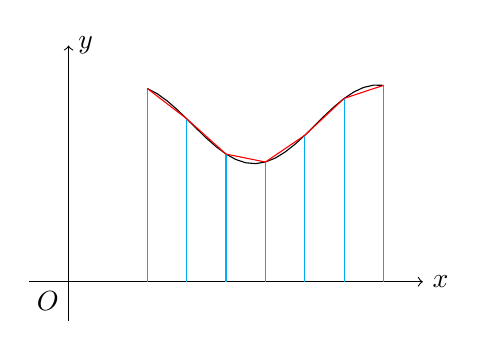
\begin{tikzpicture}
        \draw[->] (-0.5,0)--(4.5,0) node [right] {$x$};
        \draw[->] (0,-0.5)--(0,3) node [right] {$y$};
        \node at (0,0) [below left] {$O$};

        \draw[domain=1:4] plot (\x,{2+0.5*sin(2*\x r)});

        \foreach \i in {0,...,6} {
            \draw[-,cyan] (1+\i/2,0)--(1+\i/2,{2+0.5*sin((2+\i)r)});
        }
        \foreach \i in {0,...,5} {
            \draw[-,red] (1+\i/2,{2+0.5*sin((2+\i)r)})--(1.5+\i/2,{2+0.5*sin((3+\i)r)});
        }
    \end{tikzpicture}
\end{center}

记 $\mathscr{A}=\overline{\mathscr{P}}$.

\begin{lemma}
    $\mathscr{A}$ 是一个代数. 即若 $f,g\in\mathscr{A}$,则
$$
\lambda f+\mu g\in\mathscr{A},\forall\lambda,\mu\in\RR,\qquad f\cdot g\in\mathscr{A}
$$
\end{lemma}
\begin{proof}
    设 $P,Q\in\mathscr{P}$ 满足 $\norm{P-f}_\infty<\eps,\norm{Q-g}<\eps$. 则
$$
\begin{aligned}
    \norm{(\lambda P+\mu Q)-(\lambda f+\mu g)}&\le(\abs{\lambda}+\abs{\mu})\eps\\
    \norm{PQ-fg}\le\norm{P(Q-g)}+&\norm{g(P-f)}\le(\norm{P}+\norm{g})\eps\le(\norm{f}+\norm{g}+\eps)\eps
\end{aligned}
$$
\end{proof}

任给 $a\le\xi_1<\xi_2\le b$. 定义
$$
g_{\xi_1,\xi_2}(x)\triangleq\frac{x-\xi_1}{\xi_2-\xi_1}
$$

令
$$
F_{\xi_1,\xi_2}(x)\triangleq 0\wedge g_{\xi_1,\xi_2}\qquad G_{\xi_1,\xi_2}\triangleq 1\vee F_{\xi_1,\xi_2}
$$

其中 $f\wedge g\triangleq\max\set{f,g},f\vee g\triangleq\min\set{f,g}$.

\begin{center}
    \begin{tikzpicture}[scale=1.5]
        \draw[->] (-0.5,0)--(5,0) node [right] {$y$};
        \draw[->] (0,-0.5)--(0,3) node [right] {$x$};
        \node at (0,0) [below left] {$O$};
        \draw[-] (1,0.05)--(1,-0.05) node [below] {$a$};
        \draw[-] (2,0.05)--(2,-0.05) node [below] {$\xi_1$};
        \draw[-] (3,0.05)--(3,-0.05) node [below] {$\xi_2$};
        \draw[-] (4,0.05)--(4,-0.05) node [below] {$b$};
        \draw[-,dashed] (3,2)--(0,2) node [left] {$1$};
        \draw[-,dashed] (3,0)--(3,2);
        \draw[-,red] (1.7,-0.6)--(3.4,2.8) node [right] {$g_{\xi_1,\xi_2}$};
        \draw[-,blue] (-0.5,0.05)--(1.95,0.05);
        \draw[-,blue] (1.95,0.05)--(3.3,2.75) node [left] {$F_{\xi_1,\xi_2}$};
        \draw[-] (-0.5,0.1)--(1.9,0.1);
        \draw[-] (1.9,0.1)--(2.85,2);
        \draw[-] (2.85,2)--(5,2) node [right] {$G_{\xi_1,\xi_2}$};
    \end{tikzpicture}
\end{center}

\begin{lemma}
    令 $\mathscr{G}=\set{G_{\xi_1,\xi_2}|a\le\xi_1<\xi_1\le b}\cup\set{1}$.

    则 $\mathrm{span}\;\mathscr{G}=\mathscr{L}$. 即
$$
\forall f\in\mathscr{L},\exists\set{g_1,\cdots,g_m}\subset\mathscr{G},\lambda_1,\cdots,\lambda_m\in\RR,f=\sum_{j=1}^m\lambda_jg_j
$$
\end{lemma}
\begin{proof}
    直接验证.
\end{proof}

由以上引理,为了证明 Weierstrass 定理,我们仅需证明 $\mathscr{G}\subset\mathscr{A}$.

这是因为:若 $\mathscr{G}\subset\mathscr{A}$,则由 $\mathscr{A}$ 为代数知 $\mathscr{L}\subset\mathscr{A}$. 从而 $C[a,b]=\overline{\mathscr{L}}\subset\mathscr{A}$.

从而问题归结为:是否对 $\forall a\le\xi_1<\xi_2\le b$ 有 $G_{\xi_1,\xi_2}\in\mathscr{A}$.

注意到
$$
f\vee g=\frac{f+g-\abs{f-g}}{2}\qquad f\wedge g=\frac{f+g+\abs{f-g}}{2}
$$

从而由 $G_{\xi_1,\xi_2}$ 的定义方式知,如果能够证明如下的关键引理,则结论成立.

\begin{lemma}
    若 $f\in\mathscr{A}$,则 $\abs{f}\in\mathscr{A}$.
\end{lemma}
\begin{proof}
    固定 $f\in\mathscr{A}$. 设 $\norm{f}_\infty\le M$.

    断言存在 $\set{Q_n}\subset\mathscr{P}$ 使得在 $[-M,M]$ 上
$$
Q_n\rightrightarrows\abs{\cdot}
$$

    \textbf{证明:}当 $M=1$ 时,我们已经证明存在 $\set{\widetilde{Q}_n}\subset\mathscr{P}$ 使得在 $[-1,1]$ 上
$$
\widetilde{Q}_n\rightrightarrows\abs{\cdot}
$$

    令 $Q_n(y)\triangleq M\widetilde{Q}_n\left(\dfrac{y}{M}\right)$. 则 $Q_n$ 满足条件.

    \qed

    由 $\norm{f}_\infty\le M$ 以及断言知
$$
\norm{\abs{f}-Q_n(f)}_\infty\to 0
$$

    由 $f\in\mathscr{A}$ 以及 $\mathscr{A}$ 为代数知 $Q_n(f)\in\mathscr{A},\forall n\in\mathbb{N}$.

    从而上式说明 $Q_n(f)\rightrightarrows\abs{f}$. 由 $\mathscr{A}$ 闭知 $\abs{f}\in\mathscr{A}$.
\end{proof}

现任给 $a\le\xi_1<\xi_2\le b$. 则有
$$
0,g_{\xi_1,\xi_2}\in\mathscr{A}\implies F_{\xi_1,\xi_2}\in\mathscr{A}\implies G_{\xi_1,\xi_2}\in\mathscr{A}
$$

从而 Weierstrass 定理即证.

\mysubsection{Stone 定理}

我们最后在证明一个大大推广的 Weierstrass 定理:Stone 定理. 为此,我们先介绍几个概念.

\begin{definition}
    设 $\mathscr{A}$ 是一族从 $X$ 到 $\RR(\mathbb{C})$ 的函数.

    称 $\mathscr{A}$ 是一个实(复)函数代数,若 $\forall f,g\in\mathscr{A}$ 有
$$
\lambda f+\mu g\in\mathscr{A},\forall\lambda,\mu\in\RR(\mathbb{C}),\qquad f\cdot g\in\mathscr{A}
$$
\end{definition}

\begin{example}
    所有多项式的全体 $\mathscr{P}$ 为函数代数.
\end{example}

\begin{example}
    $\mathscr{A}_1\triangleq\mathrm{span}\set{e^{nx}|n\ge 0}$ 为函数代数.
\end{example}

\begin{example}
    $\mathscr{A}_1\triangleq\mathrm{span}\set{e^{inx}|n\in\mathbb{Z}}$ 为函数代数.
\end{example}

\begin{definition}
    设 $\mathscr{F}$ 是一族从 $X$ 到 $Y$ 的映射.

    称 $\mathscr{F}$ 在 $X$ 上分点,若
$$
\forall x_1,x_2\in X,x_1\ne x_2\implies\exists f\in\mathscr{F},f(x_1)\ne f(x_2)
$$
\end{definition}

\begin{example}
    $\mathscr{P}$ 在 $\RR$ 上分点,$\mathscr{A}_1$ 在 $\RR$ 上分点.

    若 $b-a<2\pi$,则 $\mathscr{A}_2$ 在 $[a,b]$ 上分点,反之不分点.
\end{example}

\begin{definition}
    设 $\mathscr{F}$ 是一族从 $X$ 到 $\RR(\mathbb{C})$ 的函数.

    称 $\mathscr{F}$ 在 $X$ 上非退化,若 $\forall x\in X,\exists f\in\mathscr{F},f(x)\ne 0$.
\end{definition}

\begin{example}
    $\set{1,x,x^2,\cdots}$ 在 $[0,1]$ 上非退化,但 $\set{x,x^2,\cdots}$ 在 $[0,1]$ 上退化.
\end{example}

\begin{lemma}
    设 $\mathscr{A}$ 是 $X$ 上的实(复)函数代数,其在 $X$ 上分点且非退化.

    则 $\forall x_1,x_2\in X,x_1\ne x_2,\forall c_1,c_2\in\RR(\mathbb{C})$ 均存在 $s\in\mathscr{A}$ 使得
$$
s(x_1)=c_1,s(x_2)=c_2
$$
\end{lemma}
\begin{proof}
    由 $\mathscr{A}$ 为代数,我们仅需考虑 $c_1=1,c_2=0$ 以及 $c_1=0,c_2=1$ 的情形.

    由对称性,我们仅需考虑 $c_1=1,c_2=0$.

    断言:存在 $\varphi\in\mathscr{A}$ 使得 $\varphi(x_1)\ne\varphi(x_2)$ 且 $\varphi(x_1)\ne 0$.

    \textbf{证明:}由 $\mathscr{A}$ 分点知:存在 $g\in\mathscr{A}$ 使得 $g(x_1)\ne g(x_2)$.

    \begin{enumerate}
        \item 若 $g(x_1)\ne 0$. 则 $\varphi=g$ 满足条件.
        
        \item 若 $g(x_1)=0$. 则 $g(x_2)\ne 0$.
        
        由 $\mathscr{A}$ 在 $X$ 上非退化,存在 $h\in\mathscr{A}$ 使得 $h(x_1)=0$.

        令 $\varphi=g+\lambda h,\lambda\ne 0$. 则只要 $\lambda$ 足够小,$\varphi$ 就满足条件.
    \end{enumerate}

    \qed

    令 $S(x)=\dfrac{\varphi(x)^2-\varphi(x_2)\varphi(x)}{\varphi(x_1)^2-\varphi(x_1)\varphi(x_2)}\in\mathscr{A}$.

    则 $S(x_1)=1,S(x_2)=0$ 满足条件.
\end{proof}

现在我们可以证明最一般的稠密性定理.

\begin{theorem}[Stone]
    设 $K$ 为紧度量空间. 设 $\mathscr{A}\subset C(K;\RR)$ 为函数代数.

    若 $\mathscr{A}$ 在 $K$ 中分点且非退化,则 $\mathscr{A}$ 在 $C(K;\RR)$ 中稠密,即 $\overline{\mathscr{A}}=C(K;\RR)$.
\end{theorem}
\begin{proof}
    首先注意到 $\mathscr{A}$ 为代数 $\implies\overline{\mathscr{A}}$ 也为代数.

    任取 $f\in C(K;\RR)$. 由 $K$ 紧知 $\norm{f}_\infty\le M$. 从而利用上一定理的证明可得:
$$
f\in\mathscr{A}\implies\abs{f}\in\overline{\mathscr{A}}
$$

    进而有:若 $f,g\in\mathscr{A}$,则
$$
f\wedge g=\frac{f+g+\abs{f-g}}{2}\in\overline{\mathscr{A}}\qquad f\vee g=\frac{f+g-\abs{f-g}}{2}\in\overline{\mathscr{A}}
$$

    归纳的有
$$
f_1,\cdots,f_n\in\mathscr{A}\implies f_1\wedge\cdots\wedge f_n,f_1\vee\cdots\vee f_n\in\overline{\mathscr{A}}
$$
\end{proof}